%%%%%%%%%%%%%%%%%%%%%%%%%%%%%%%%%%%%%%%%%%
%Copyright (C) 2018-2020  YuZJLab
%This program is free software: you can redistribute it and/or modify
%it under the terms of the GNU General Public License as published by
%the Free Software Foundation, either version 3 of the License, or
%(at your option) any later version.
%This program is distributed in the hope that it will be useful,
%but WITHOUT ANY WARRANTY; without even the implied warranty of
%MERCHANTABILITY or FITNESS FOR A PARTICULAR PURPOSE.  See the
%GNU General Public License for more details.
%You should have received a copy of the GNU General Public License
%along with this program.  If not, see <https://www.gnu.org/licenses/>.
%%%%%%%%%%%%%%%%%%%%%%%%%%%%%%%%%%%%%%%%%%
\documentclass{book}
\usepackage{xeCJK} %中文支持
\setCJKsansfont{SourceHanSansCN-ExtraLight.otf}
\setCJKmonofont{SourceCodePro-Light.otf}
\setCJKmainfont{SourceHanSerifSC-ExtraLight.otf}
\setCJKfamilyfont{bolded}{SourceHanSansSC-Bold.otf}
\renewcommand{\bf}{\CJKfamily{bolded}}
\newcommand{\normalall}{\normalsize\normalfont\normalcolor}  
\usepackage{color}
\usepackage{graphicx}  %生成图片
\usepackage{geometry} %设置页面排版
\geometry{top=0.5in, bottom=0.5in, left=0.5in, right=0.5in, papersize={21cm,29.7cm}}
\usepackage[super]{nth} %生成序数词
\bibliographystyle{unsrt}
\usepackage{metalogo} %生成TeX标志
\usepackage{texnames} %生成TeX标志
\usepackage{fancybox} %生成带阴影的盒子
\shadowsize=2pt %配置盒子
\usepackage{shorttoc}
\usepackage{flafter}%使得所有浮动体不能被放置在其浮动环境之前
\usepackage{picinpar} %生成文本环绕
\usepackage{indentfirst}%生成段落
\usepackage[toc]{multitoc}%双栏目录
\usepackage{amssymb}%显示方块
\makeatletter\renewcommand{\verbatim@font}{\footnotesize \color{blue}\texttt} \makeatletter%修改verbatim环境格式
 %生成章节中文名和盒子
\renewcommand{\thechapter}{\arabic{chapter}}
\renewcommand{\thesection}{\arabic{chapter}.\arabic{section}}
\renewcommand{\thesubsection}{\arabic{chapter}.\arabic{section}.\arabic{subsection}}
\renewcommand{\thesubsubsection}{\arabic{chapter}.\arabic{section}.\arabic{subsection}.\arabic{subsubsection}}
\usepackage{titlesec}
\renewcommand{\bibname}{参考文献}
\renewcommand{\contentsname}{目录}
\renewcommand{\appendixname}{附录}
\titleformat{\chapter}[frame]{\bf \Huge}{\small 第 \thechapter 部分}{0pt}{}
\titleformat{\section}[frame]{\bf  \LARGE}{\small 第 \thesection 章}{0pt}{}
\titleformat{\subsection}[frame]{\bf  \Large}{\small  第\thesubsection 节}{0pt}{}
\titleformat{\subsubsection}[frame]{\bf \large}{\small 第\thesubsubsection 小节}{0pt}{}
\linespread{1.2} %行距命令
\usepackage{eso-pic}%背景图像命令
\usepackage[backref]{hyperref} %生成书签,这个应被放在末尾
\hypersetup{hidelinks,bookmarks=true,bookmarksopen=true,pdftitle=EMACS 26.2中文手册,pdfauthor=YuZJ}
\begin{document}
\setcounter{tocdepth}{5}
\begin{titlepage}	
\AddToShipoutPictureBG*{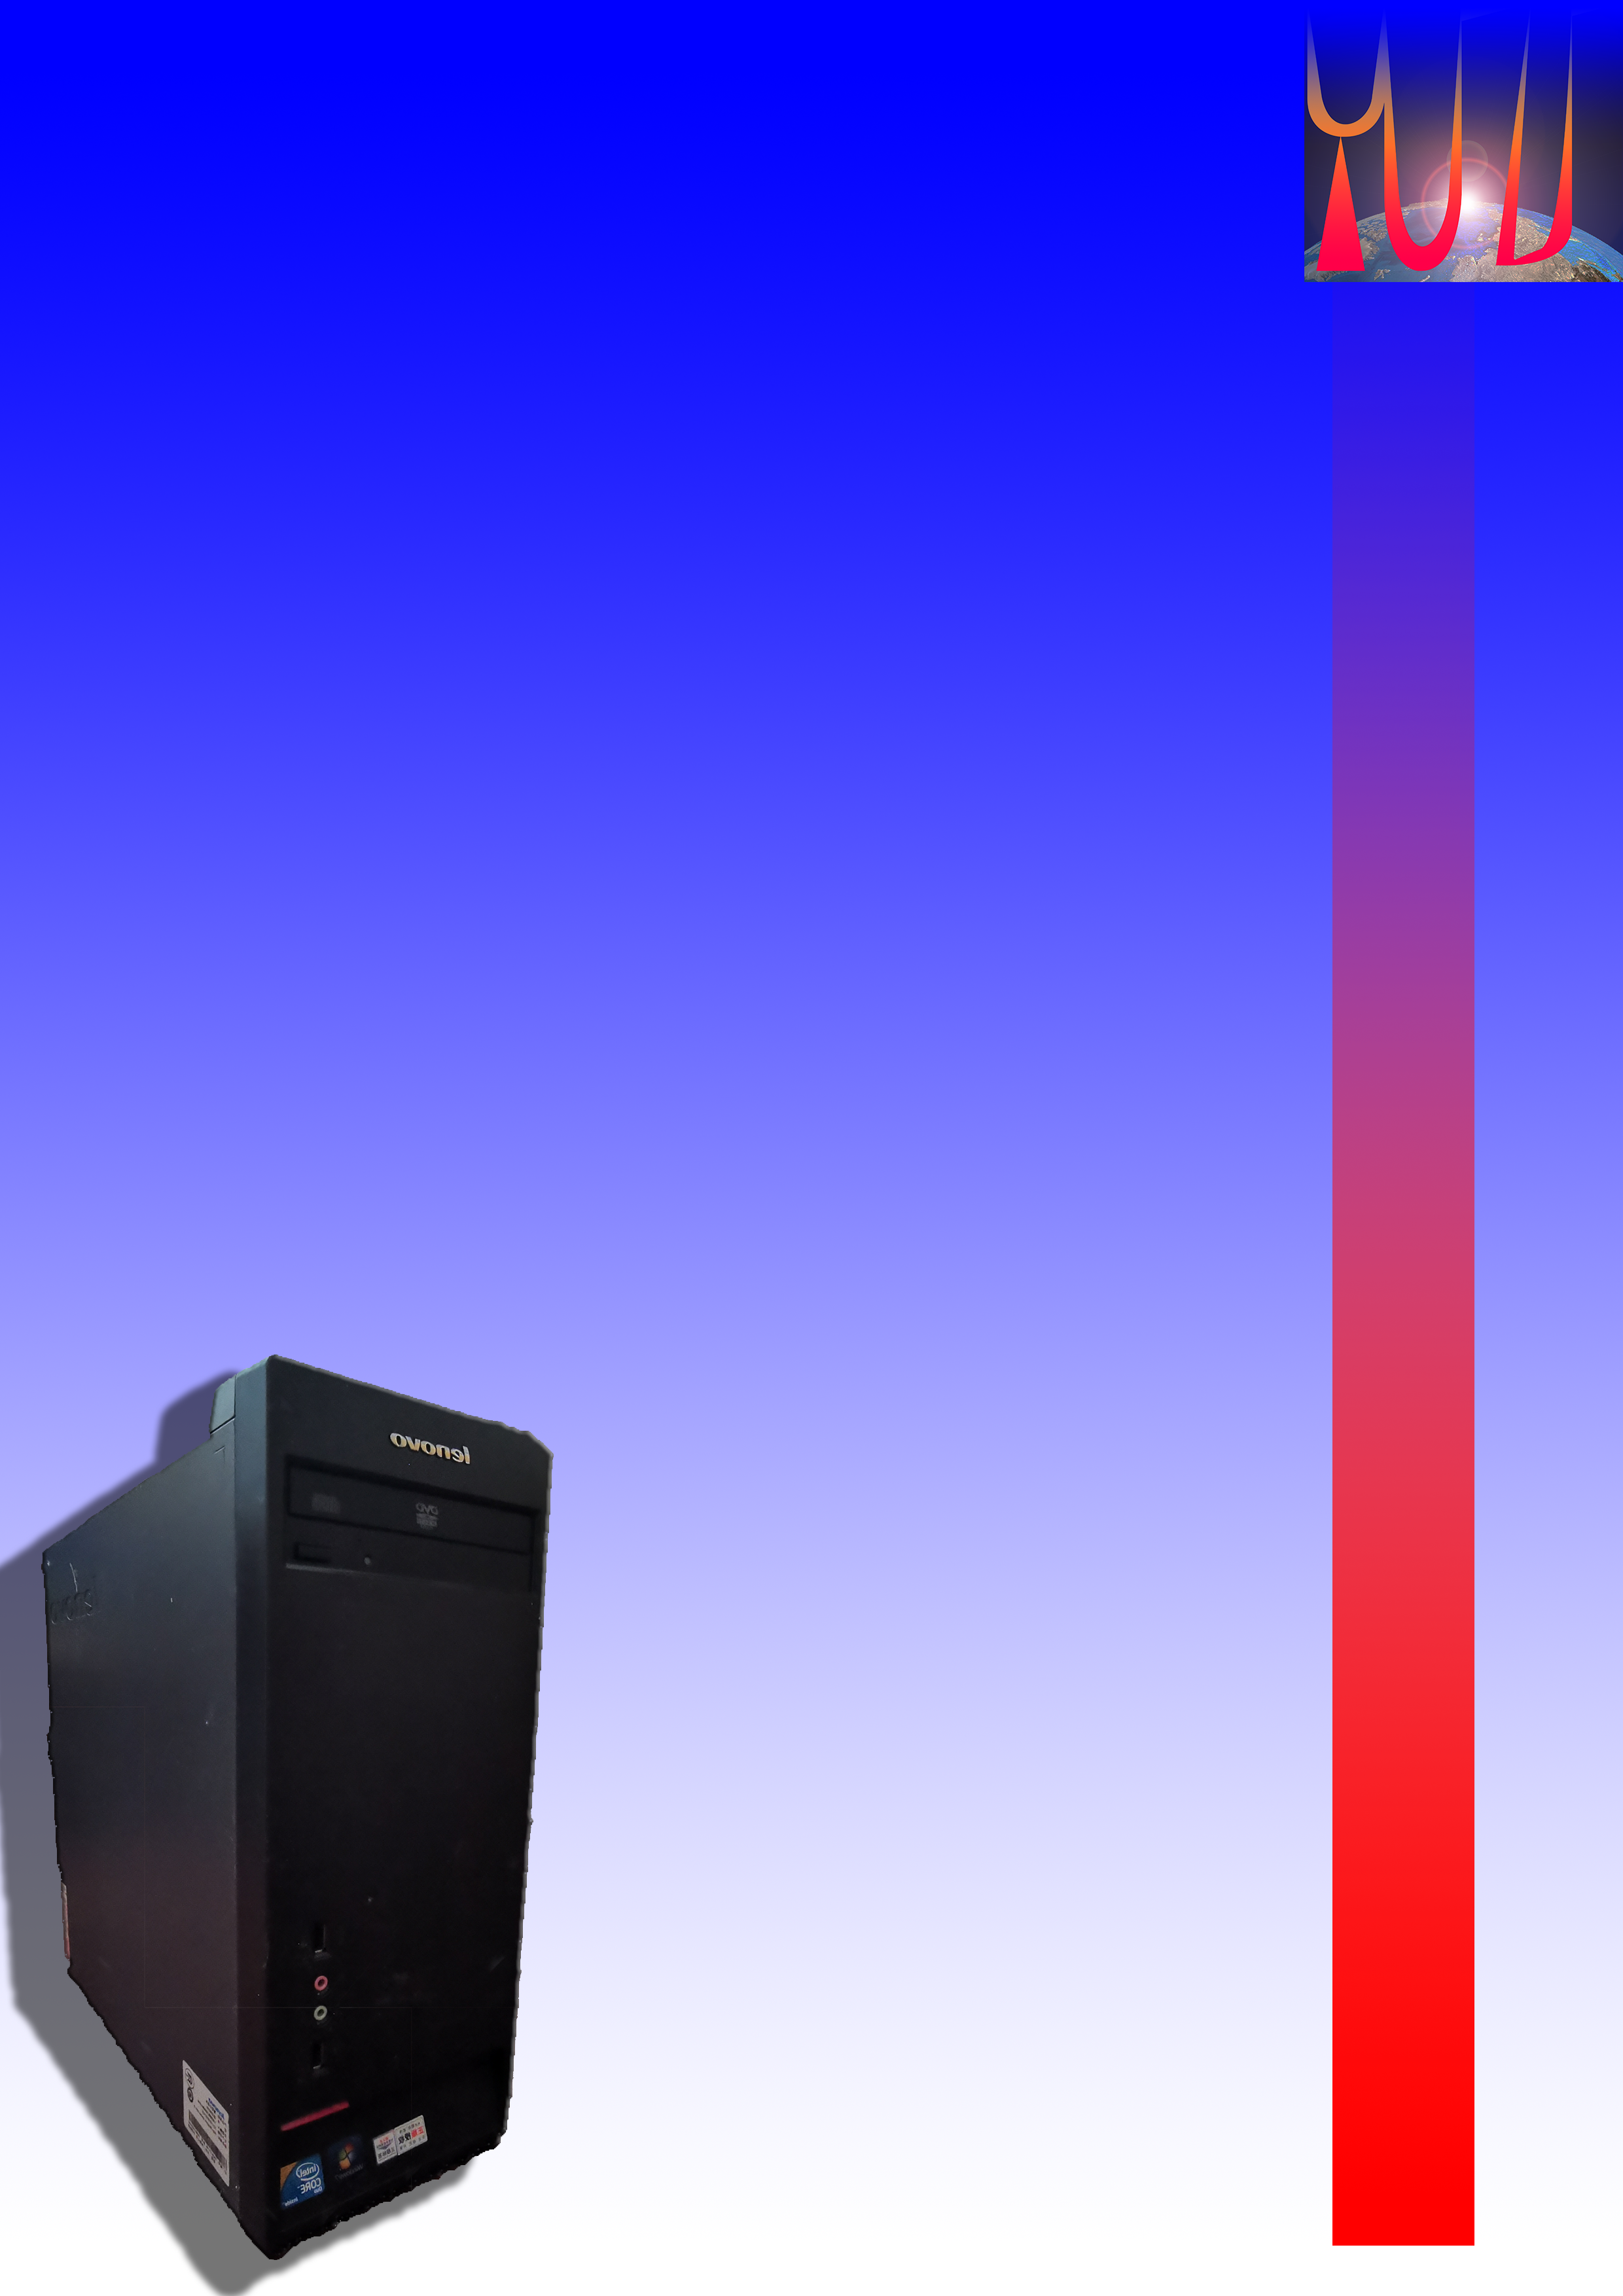
\includegraphics[width=21cm,height=29.7cm]{pic/face.png}}
{\color{white}{
\vspace*{10mm}
\begin{center}
\doublebox{\parbox{18cm}{
\begin{center}	
\Ovalbox{\Huge \bf EMACS 26.2中文手册\normalsize}\\\vspace*{5mm}\bf \large 作者:YuZJ \\\vspace*{5mm} 编译日期:\today	
\end{center}}}
\end{center}}}
\vspace*{25mm}\normalall
\shadowbox{\parbox[t]{8cm}{{\color{white}{【简介】}}}}
\end{titlepage}
\begin{center}
	\Huge \bf 【版本号】 \normalall
\end{center}
\shorttoc{简明目录}{1}
\tableofcontents
\chapter{The Organization of the Screen:屏幕的组织结构}
On a graphical display, such as on GNU/Linux using the X Window System, Emacs occupies
a graphical window. On a text terminal, Emacs occupies the entire terminal screen. We
will use the term frame to mean a graphical window or terminal screen occupied by Emacs.
Emacs behaves very similarly on both kinds of frames. It normally starts out with just one
frame, but you can create additional frames if you wish (see Chapter 18 [Frames]).
\par
在一个图形界面(例如,使用X Windows系统的GNU/Linux操作系统)中,Emacs占用了一个图形窗口(Window)。在一个文本终端中,Emacs占用了一整个终端屏幕。我们将会使用“窗体”(Frame)表示Emacs占用的图形窗体或终端屏幕。Emacs在这两种窗体下表现十分相似\footnote{译注:虽然我不这么认为}。一般情况下Emacs在启动时创建一个窗体,但是你可以按照你的意愿创建另外的窗体(参见第18章【窗体】)。\par
Each frame consists of several distinct regions. At the top of the frame is a menu bar,
which allows you to access commands via a series of menus. On a graphical display, directly
below the menu bar is a tool bar, a row of icons that perform editing commands when you
click on them. At the very bottom of the frame is an echo area, where informative messages
are displayed and where you enter information when Emacs asks for it.
\par
Emacs窗体包括多个区分明显的区域。在窗体的最顶端是菜单栏(Menu Bar),它允许你通过一系列菜单访问命令。在一个图形界面上,菜单栏下方是工具栏(Tool Bar)。它由一系列图标构成,当你单击它是它将执行编辑命令。回显区(Echo Area)窗体的最底端,用于显示Emacs的提示信息或者当Emacs需要你输入时键入信息。\par
The main area of the frame, below the tool bar (if one exists) and above the echo area, is
called the window. Henceforth in this manual, we will use the word “window” in this sense.
Graphical display systems commonly use the word “window” with a different meaning; but,
as stated above, we refer to those graphical windows as “frames”.
\par
在一个Emacs窗体中,位于工具栏(如果存在的话)以及回显区的大块区域称为窗格(Window)。此后我们将会使用“窗格”来表示这个意思。图形界面系统一般会使用“窗口”(Window)来表示不同的意思;但是,正如已经声明的一样,我们将称这些图形界面窗口为“窗体”(Frame)。\par
An Emacs window is where the buffer—the text or other graphics you are editing or
viewing—is displayed. On a graphical display, the window possesses a scroll bar on one
side, which can be used to scroll through the buffer. The last line of the window is a mode
line. This displays various information about what is going on in the buffer, such as whether
there are unsaved changes, the editing modes that are in use, the current line number, and
so forth.
\par
缓冲区(Buffer)——文本、图像以及其他你正在编辑或浏览的东西所显示的地方——位于Emacs窗口。在一个图形界面上,窗格\footnote{译注:是“Window”。此后窗格一律称“Window”,窗体一律称“Frame”。窗口?那是什么东西?}拥有一个纵向的滚动条用于滚动显示整个缓冲区。窗格的最底端一栏(在终端界面下是一行文字)称为状态栏(Mode Line),用于显示关于缓冲区中正在进行的操作的的信息,比如说是否有未保存的改变,正在使用的编辑模式(Editing Mode),当前的行号等等。\par
When you start Emacs, there is normally only one window in the frame. However, you
can subdivide this window horizontally or vertically to create multiple windows, each of
which can independently display a buffer (see Chapter 17 [Windows]).
\par
通常情况下,当你启动Emacs的时候,一个窗体中只有一个窗格。但是,你可以将这个窗格水平或竖直地分为多个窗格,它们各自独立地显示一个缓冲区(参见第17章【窗格】)。\par
At any time, one window is the selected window. On a graphical display, the selected
window shows a more prominent cursor (usually solid and blinking); other windows show a
less prominent cursor (usually a hollow box). On a text terminal, there is only one cursor,
which is shown in the selected window. The buffer displayed in the selected window is
called the current buffer, and it is where editing happens. Most Emacs commands implicitly
apply to the current buffer; the text displayed in unselected windows is mostly visible for
reference. If you use multiple frames on a graphical display, selecting a particular frame
selects a window in that frame.\par
在任何时候,有且仅有一个窗格是活动窗格(Selected Window)。在一个图形界面下,活动窗格显示一个更加明显的光标(Crusor)(一般是闪动的黑色方块“$\blacksquare$”);其它窗格显示一个不明显的光标(一般是空心方块“$\square$”)。终端界面只将在活动窗格显示一个光标。在活动窗格显示的缓冲区称为活动缓冲区(“Selected Buffer”)并且就是正在被编辑的缓冲区。大部分Emacs命令含蓄地作用于活动缓冲区;在非活动的缓冲区中显示的文字仅仅为参考而显示。如果你使用多窗体的图形界面,选择一个窗体再选择一个窗格。
\begin{center}
	\includegraphics[scale=0.4]{pic/Emacs-Terminal-Defaut}
\end{center}

\appendix
\input{GPL}
%%%%%%%%%%%%%%%%%%%%%%%%%%%%%%%%%%%%%%%%%%
%Copyright (C) 2018-2020  YuZJLab
%This program is free software: you can redistribute it and/or modify
%it under the terms of the GNU General Public License as published by
%the Free Software Foundation, either version 3 of the License, or
%(at your option) any later version.
%This program is distributed in the hope that it will be useful,
%but WITHOUT ANY WARRANTY; without even the implied warranty of
%MERCHANTABILITY or FITNESS FOR A PARTICULAR PURPOSE.  See the
%GNU General Public License for more details.
%You should have received a copy of the GNU General Public License
%along with this program.  If not, see <https://www.gnu.org/licenses/>.
%%%%%%%%%%%%%%%%%%%%%%%%%%%%%%%%%%%%%%%%%%
\chapter{The GNU Manifesto}
The GNU Manifesto (which appears below) was written by \href{http://www.stallman.org/}{Richard Stallman} in 1985 to ask for support in developing the GNU operating system. Part of the text was taken from the original announcement of 1983. Through 1987, it was updated in minor ways to account for developments; since then, it seems best to leave it unchanged.\par
Since that time, we have learned about certain common misunderstandings that different wording could help avoid. Footnotes added since 1993 help clarify these points.\par
If you want to install the GNU/Linux system, we recommend you use one of the \href{http://www.gnu.org/distros/}{100\% free software GNU/Linux distributions}. For how to contribute, see \url{http://www.gnu.org/help}.\par
The GNU Project is part of the Free Software Movement, a campaign for \href{http://www.gnu.org/philosophy/free-sw.html}{freedom for users of software}. It is a mistake to associate GNU with the term “open source”—that term was coined in 1998 by people who disagree with the Free Software Movement's ethical values. They use it to promote an \href{http://www.gnu.org/philosophy/open-source-misses-the-point.html}{amoral approach} to the same field.
\section{What's GNU? Gnu's Not Unix!}
GNU, which stands for Gnu's Not Unix, is the name for the complete Unix-compatible software system which I am writing so that I can give it away free to everyone who can use it.\footnote{The wording here was careless. The intention was that nobody would have to pay for permission to use the GNU system. But the words don't make this clear, and people often interpret them as saying that copies of GNU should always be distributed at little or no charge. That was never the intent; later on, the manifesto mentions the possibility of companies providing the service of distribution for a profit. Subsequently I have learned to distinguish carefully between “free” in the sense of freedom and “free” in the sense of price. Free software is software that users have the freedom to distribute and change. Some users may obtain copies at no charge, while others pay to obtain copies—and if the funds help support improving the software, so much the better. The important thing is that everyone who has a copy has the freedom to cooperate with others in using it.}  Several other volunteers are helping me. Contributions of time, money, programs and equipment are greatly needed.\par
So far we have an Emacs text editor with Lisp for writing editor commands, a source level debugger, a yacc-compatible parser generator, a linker, and around 35 utilities. A shell (command interpreter) is nearly completed. A new portable optimizing C compiler has compiled itself and may be released this year. An initial kernel exists but many more features are needed to emulate Unix. When the kernel and compiler are finished, it will be possible to distribute a GNU system suitable for program development. We will use TeX as our text formatter, but an nroff is being worked on. We will use the free, portable X Window System as well. After this we will add a portable Common Lisp, an Empire game, a spreadsheet, and hundreds of other things, plus online documentation. We hope to supply, eventually, everything useful that normally comes with a Unix system, and more.\par
GNU will be able to run Unix programs, but will not be identical to Unix. We will make all improvements that are convenient, based on our experience with other operating systems. In particular, we plan to have longer file names, file version numbers, a crashproof file system, file name completion perhaps, terminal-independent display support, and perhaps eventually a Lisp-based window system through which several Lisp programs and ordinary Unix programs can share a screen. Both C and Lisp will be available as system programming languages. We will try to support UUCP, MIT Chaosnet, and Internet protocols for communication.\par
GNU is aimed initially at machines in the 68000/16000 class with virtual memory, because they are the easiest machines to make it run on. The extra effort to make it run on smaller machines will be left to someone who wants to use it on them.\par
To avoid horrible confusion, please pronounce the g in the word “GNU” when it is the name of this project.
\section{Why I Must Write GNU}
I consider that the Golden Rule requires that if I like a program I must share it with other people who like it. Software sellers want to divide the users and conquer them, making each user agree not to share with others. I refuse to break solidarity with other users in this way. I cannot in good conscience sign a nondisclosure agreement or a software license agreement. For years I worked within the Artificial Intelligence Lab to resist such tendencies and other inhospitalities, but eventually they had gone too far: I could not remain in an institution where such things are done for me against my will.\par
So that I can continue to use computers without dishonor, I have decided to put together a sufficient body of free software so that I will be able to get along without any software that is not free. I have resigned from the AI Lab to deny MIT any legal excuse to prevent me from giving GNU away.\footnote{The expression “give away” is another indication that I had not yet clearly separated the issue of price from that of freedom. We now recommend avoiding this expression when talking about free software. See “\href{http://www.gnu.org/philosophy/words-to-avoid.html\#GiveAwaySoftware}{Confusing Words and Phrases}” for more explanation.}
\section{Why GNU Will Be Compatible with Unix}
Unix is not my ideal system, but it is not too bad. The essential features of Unix seem to be good ones, and I think I can fill in what Unix lacks without spoiling them. And a system compatible with Unix would be convenient for many other people to adopt.
\section{How GNU Will Be Available}
GNU is not in the public domain. Everyone will be permitted to modify and redistribute GNU, but no distributor will be allowed to restrict its further redistribution. That is to say, \href{http://www.gnu.org/philosophy/categories.html\#ProprietarySoftware}{proprietary} modifications will not be allowed. I want to make sure that all versions of GNU remain free.
\section{Why Many Other Programmers Want to Help}
I have found many other programmers who are excited about GNU and want to help.
Many programmers are unhappy about the commercialization of system software. It may enable them to make more money, but it requires them to feel in conflict with other programmers in general rather than feel as comrades. The fundamental act of friendship among programmers is the sharing of programs; marketing arrangements now typically used essentially forbid programmers to treat others as friends. The purchaser of software must choose between friendship and obeying the law. Naturally, many decide that friendship is more important. But those who believe in law often do not feel at ease with either choice. They become cynical and think that programming is just a way of making money.\par
By working on and using GNU rather than proprietary programs, we can be hospitable to everyone and obey the law. In addition, GNU serves as an example to inspire and a banner to rally others to join us in sharing. This can give us a feeling of harmony which is impossible if we use software that is not free. For about half the programmers I talk to, this is an important happiness that money cannot replace.
\section{How You Can Contribute}
(Nowadays, for software tasks to work on, see the \href{http://fsf.org/campaigns/priority-projects}{High Priority Projects list} and the \href{http://savannah.gnu.org/people/?type_id=1}{GNU Help Wanted list}, the general task list for GNU software packages. For other ways to help, see the \href{http://www.gnu.org/help/help.html}{guide to helping the GNU operating system}.)\par
I am asking computer manufacturers for donations of machines and money. I'm asking individuals for donations of programs and work.\par
One consequence you can expect if you donate machines is that GNU will run on them at an early date. The machines should be complete, ready to use systems, approved for use in a residential area, and not in need of sophisticated cooling or power.\par
I have found very many programmers eager to contribute part-time work for GNU. For most projects, such part-time distributed work would be very hard to coordinate; the independently written parts would not work together. But for the particular task of replacing Unix, this problem is absent. A complete Unix system contains hundreds of utility programs, each of which is documented separately. Most interface specifications are fixed by Unix compatibility. If each contributor can write a compatible replacement for a single Unix utility, and make it work properly in place of the original on a Unix system, then these utilities will work right when put together. Even allowing for Murphy to create a few unexpected problems, assembling these components will be a feasible task. (The kernel will require closer communication and will be worked on by a small, tight group.)\par
If I get donations of money, I may be able to hire a few people full or part time. The salary won't be high by programmers' standards, but I'm looking for people for whom building community spirit is as important as making money. I view this as a way of enabling dedicated people to devote their full energies to working on GNU by sparing them the need to make a living in another way.
\section{Why All Computer Users Will Benefit}
Once GNU is written, everyone will be able to obtain good system software free, just like air.\footnote{This is another place I failed to distinguish carefully between the two different meanings of “free”. The statement as it stands is not false—you can get copies of GNU software at no charge, from your friends or over the net. But it does suggest the wrong idea.}\par
This means much more than just saving everyone the price of a Unix license. It means that much wasteful duplication of system programming effort will be avoided. This effort can go instead into advancing the state of the art.\par
Complete system sources will be available to everyone. As a result, a user who needs changes in the system will always be free to make them himself, or hire any available programmer or company to make them for him. Users will no longer be at the mercy of one programmer or company which owns the sources and is in sole position to make changes.\par
Schools will be able to provide a much more educational environment by encouraging all students to study and improve the system code. Harvard's computer lab used to have the policy that no program could be installed on the system if its sources were not on public display, and upheld it by actually refusing to install certain programs. I was very much inspired by this.\par
Finally, the overhead of considering who owns the system software and what one is or is not entitled to do with it will be lifted.\par
Arrangements to make people pay for using a program, including licensing of copies, always incur a tremendous cost to society through the cumbersome mechanisms necessary to figure out how much (that is, which programs) a person must pay for. And only a police state can force everyone to obey them. Consider a space station where air must be manufactured at great cost: charging each breather per liter of air may be fair, but wearing the metered gas mask all day and all night is intolerable even if everyone can afford to pay the air bill. And the TV cameras everywhere to see if you ever take the mask off are outrageous. It's better to support the air plant with a head tax and chuck the masks.\par
Copying all or parts of a program is as natural to a programmer as breathing, and as productive. It ought to be as free.
\section{Some Easily Rebutted Objections to GNU's Goals}
\textbf{“Nobody will use it if it is free, because that means they can't rely on any support.”}\par
\textbf{“You have to charge for the program to pay for providing the support.”}\par
If people would rather pay for GNU plus service than get GNU free without service, a company to provide just service to people who have obtained GNU free ought to be profitable.\footnote{Several such companies now exist.}\par
We must distinguish between support in the form of real programming work and mere handholding. The former is something one cannot rely on from a software vendor. If your problem is not shared by enough people, the vendor will tell you to get lost.\par
If your business needs to be able to rely on support, the only way is to have all the necessary sources and tools. Then you can hire any available person to fix your problem; you are not at the mercy of any individual. With Unix, the price of sources puts this out of consideration for most businesses. With GNU this will be easy. It is still possible for there to be no available competent person, but this problem cannot be blamed on distribution arrangements. GNU does not eliminate all the world's problems, only some of them.\par
Meanwhile, the users who know nothing about computers need handholding: doing things for them which they could easily do themselves but don't know how.\par
Such services could be provided by companies that sell just handholding and repair service. If it is true that users would rather spend money and get a product with service, they will also be willing to buy the service having got the product free. The service companies will compete in quality and price; users will not be tied to any particular one. Meanwhile, those of us who don't need the service should be able to use the program without paying for the service.\par
\textbf{“You cannot reach many people without advertising, and you must charge for the program to support that.”}\par
\textbf{“It's no use advertising a program people can get free.”}\par
There are various forms of free or very cheap publicity that can be used to inform numbers of computer users about something like GNU. But it may be true that one can reach more microcomputer users with advertising. If this is really so, a business which advertises the service of copying and mailing GNU for a fee ought to be successful enough to pay for its advertising and more. This way, only the users who benefit from the advertising pay for it.\par
On the other hand, if many people get GNU from their friends, and such companies don't succeed, this will show that advertising was not really necessary to spread GNU. Why is it that free market advocates don't want to let the free market decide this?\footnote{Although it is a charity rather than a company, the Free Software Foundation for 10 years raised most of its funds from its distribution service. You can \href{http://www.gnu.org/order/order.html}{order things from the FSF} to support its work. }\par
\textbf{“My company needs a proprietary operating system to get a competitive edge.”}\par
GNU will remove operating system software from the realm of competition. You will not be able to get an edge in this area, but neither will your competitors be able to get an edge over you. You and they will compete in other areas, while benefiting mutually in this one. If your business is selling an operating system, you will not like GNU, but that's tough on you. If your business is something else, GNU can save you from being pushed into the expensive business of selling operating systems.\par
I would like to see GNU development supported by gifts from many manufacturers and users, reducing the cost to each.\footnote{A group of computer companies pooled funds around 1991 to support maintenance of the GNU C Compiler.}\par
\textbf{“Don't programmers deserve a reward for their creativity?”}\par
If anything deserves a reward, it is social contribution. Creativity can be a social contribution, but only in so far as society is free to use the results. If programmers deserve to be rewarded for creating innovative programs, by the same token they deserve to be punished if they restrict the use of these programs.\par
\textbf{“Shouldn't a programmer be able to ask for a reward for his creativity?”}\par
There is nothing wrong with wanting pay for work, or seeking to maximize one's income, as long as one does not use means that are destructive. But the means customary in the field of software today are based on destruction.\par
Extracting money from users of a program by restricting their use of it is destructive because the restrictions reduce the amount and the ways that the program can be used. This reduces the amount of wealth that humanity derives from the program. When there is a deliberate choice to restrict, the harmful consequences are deliberate destruction.\par
The reason a good citizen does not use such destructive means to become wealthier is that, if everyone did so, we would all become poorer from the mutual destructiveness. This is Kantian ethics; or, the Golden Rule. Since I do not like the consequences that result if everyone hoards information, I am required to consider it wrong for one to do so. Specifically, the desire to be rewarded for one's creativity does not justify depriving the world in general of all or part of that creativity.\par
\textbf{“Won't programmers starve?”}\par
I could answer that nobody is forced to be a programmer. Most of us cannot manage to get any money for standing on the street and making faces. But we are not, as a result, condemned to spend our lives standing on the street making faces, and starving. We do something else.\par
But that is the wrong answer because it accepts the questioner's implicit assumption: that without ownership of software, programmers cannot possibly be paid a cent. Supposedly it is all or nothing.\par
The real reason programmers will not starve is that it will still be possible for them to get paid for programming; just not paid as much as now.\par
Restricting copying is not the only basis for business in software. It is the most common basis\footnote{I think I was mistaken in saying that proprietary software was the most common basis for making money in software. It seems that actually the most common business model was and is development of custom software. That does not offer the possibility of collecting rents, so the business has to keep doing real work in order to keep getting income. The custom software business would continue to exist, more or less unchanged, in a free software world. Therefore, I no longer expect that most paid programmers would earn less in a free software world.} because it brings in the most money. If it were prohibited, or rejected by the customer, software business would move to other bases of organization which are now used less often. There are always numerous ways to organize any kind of business.\par
Probably programming will not be as lucrative on the new basis as it is now. But that is not an argument against the change. It is not considered an injustice that sales clerks make the salaries that they now do. If programmers made the same, that would not be an injustice either. (In practice they would still make considerably more than that.)\par
\textbf{“Don't people have a right to control how their creativity is used?”}\par
“Control over the use of one's ideas” really constitutes control over other people's lives; and it is usually used to make their lives more difficult.\par
People who have studied the issue of intellectual property rights\footnote{In the 1980s I had not yet realized how confusing it was to speak of “the issue” of “intellectual property”. That term is obviously biased; more subtle is the fact that it lumps together various disparate laws which raise very different issues. Nowadays I urge people to reject the term “intellectual property” entirely, lest it lead others to suppose that those laws form one coherent issue. The way to be clear is to discuss patents, copyrights, and trademarks separately. See \href{http://www.gnu.org/philosophy/not-ipr.html}{further explanation} of how this term spreads confusion and bias.} carefully (such as lawyers) say that there is no intrinsic right to intellectual property. The kinds of supposed intellectual property rights that the government recognizes were created by specific acts of legislation for specific purposes.\par
For example, the patent system was established to encourage inventors to disclose the details of their inventions. Its purpose was to help society rather than to help inventors. At the time, the life span of 17 years for a patent was short compared with the rate of advance of the state of the art. Since patents are an issue only among manufacturers, for whom the cost and effort of a license agreement are small compared with setting up production, the patents often do not do much harm. They do not obstruct most individuals who use patented products.\par
The idea of copyright did not exist in ancient times, when authors frequently copied other authors at length in works of nonfiction. This practice was useful, and is the only way many authors' works have survived even in part. The copyright system was created expressly for the purpose of encouraging authorship. In the domain for which it was invented—books, which could be copied economically only on a printing press—it did little harm, and did not obstruct most of the individuals who read the books.\par
All intellectual property rights are just licenses granted by society because it was thought, rightly or wrongly, that society as a whole would benefit by granting them. But in any particular situation, we have to ask: are we really better off granting such license? What kind of act are we licensing a person to do?\par
The case of programs today is very different from that of books a hundred years ago. The fact that the easiest way to copy a program is from one neighbor to another, the fact that a program has both source code and object code which are distinct, and the fact that a program is used rather than read and enjoyed, combine to create a situation in which a person who enforces a copyright is harming society as a whole both materially and spiritually; in which a person should not do so regardless of whether the law enables him to.\par
\textbf{“Competition makes things get done better.”}\par
The paradigm of competition is a race: by rewarding the winner, we encourage everyone to run faster. When capitalism really works this way, it does a good job; but its defenders are wrong in assuming it always works this way. If the runners forget why the reward is offered and become intent on winning, no matter how, they may find other strategies—such as, attacking other runners. If the runners get into a fist fight, they will all finish late.\par
Proprietary and secret software is the moral equivalent of runners in a fist fight. Sad to say, the only referee we've got does not seem to object to fights; he just regulates them (“For every ten yards you run, you can fire one shot”). He really ought to break them up, and penalize runners for even trying to fight.\par
\textbf{“Won't everyone stop programming without a monetary incentive?”}\par
Actually, many people will program with absolutely no monetary incentive. Programming has an irresistible fascination for some people, usually the people who are best at it. There is no shortage of professional musicians who keep at it even though they have no hope of making a living that way.\par
But really this question, though commonly asked, is not appropriate to the situation. Pay for programmers will not disappear, only become less. So the right question is, will anyone program with a reduced monetary incentive? My experience shows that they will.\par
For more than ten years, many of the world's best programmers worked at the Artificial Intelligence Lab for far less money than they could have had anywhere else. They got many kinds of nonmonetary rewards: fame and appreciation, for example. And creativity is also fun, a reward in itself.\par
Then most of them left when offered a chance to do the same interesting work for a lot of money.\par
What the facts show is that people will program for reasons other than riches; but if given a chance to make a lot of money as well, they will come to expect and demand it. Low-paying organizations do poorly in competition with high-paying ones, but they do not have to do badly if the high-paying ones are banned.\par
\textbf{“We need the programmers desperately. If they demand that we stop helping our neighbors, we have to obey.”}\par
You're never so desperate that you have to obey this sort of demand. Remember: millions for defense, but not a cent for tribute!\par
\textbf{“Programmers need to make a living somehow.”}\par
In the short run, this is true. However, there are plenty of ways that programmers could make a living without selling the right to use a program. This way is customary now because it brings programmers and businessmen the most money, not because it is the only way to make a living. It is easy to find other ways if you want to find them. Here are a number of examples.\par
A manufacturer introducing a new computer will pay for the porting of operating systems onto the new hardware.\par
The sale of teaching, handholding and maintenance services could also employ programmers.\par
People with new ideas could distribute programs as freeware\footnote{Subsequently we learned to distinguish between “free software” and “freeware”. The term “freeware” means software you are free to redistribute, but usually you are not free to study and change the source code, so most of it is not free software. See “\href{http://www.gnu.org/philosophy/words-to-avoid.html\#Freeware}{Confusing Words and Phrases}” for more explanation.}, asking for donations from satisfied users, or selling handholding services. I have met people who are already working this way successfully.\par
Users with related needs can form users' groups, and pay dues. A group would contract with programming companies to write programs that the group's members would like to use.\par
All sorts of development can be funded with a Software Tax:\par
Suppose everyone who buys a computer has to pay x percent of the price as a software tax. The government gives this to an agency like the NSF to spend on software development.\par
But if the computer buyer makes a donation to software development himself, he can take a credit against the tax. He can donate to the project of his own choosing—often, chosen because he hopes to use the results when it is done. He can take a credit for any amount of donation up to the total tax he had to pay.\par
The total tax rate could be decided by a vote of the payers of the tax, weighted according to the amount they will be taxed on.\par
\textbf{The consequences:}\par
The computer-using community supports software development.\par
This community decides what level of support is needed.\par
Users who care which projects their share is spent on can choose this for themselves.\par
In the long run, making programs free is a step toward the postscarcity world, where nobody will have to work very hard just to make a living. People will be free to devote themselves to activities that are fun, such as programming, after spending the necessary ten hours a week on required tasks such as legislation, family counseling, robot repair and asteroid prospecting. There will be no need to be able to make a living from programming.\par
We have already greatly reduced the amount of work that the whole society must do for its actual productivity, but only a little of this has translated itself into leisure for workers because much nonproductive activity is required to accompany productive activity. The main causes of this are bureaucracy and isometric struggles against competition. Free software will greatly reduce these drains in the area of software production. We must do this, in order for technical gains in productivity to translate into less work for us.
\chapter{GNU宣言}
\cite{gnum}
GNU宣言\footnote{注意,有些脚注是由GNU CTT加的。}(如下所示)由\href{http://www.stallman.org/}{Richard Stallman}在1985年撰写,用来请求大家支持GNU操作系统的开发。其部分文本摘自1983年撰写的初始声明。直到1987年,因为开发的原因它时时小有更改;那时起,看起来最好是保持它不再改变。\par
时过境迁,我们认识到使用不同的措辞可以避免一些常见的误解。从1993年起,我们添加了脚注来澄清这些问题。\par
如果你想安装GNU/Linux系统,我们建议你使用\href{http://www.gnu.org/distros}{100\%自由的GNU/Linux发行版}之一。如果你想做出贡献,请参看\url{http://www.gnu.org/help/help.html}。\par
GNU工程是自由软件运动的一部分,该运动旨在\href{http://www.gnu.org/philosophy/free-sw.html}{捍卫软件用户的自由}。把GNU和“开源”一词联系在一起是错误的—该词汇是1998年由一些不赞同自由软件运动之道德价值的人士发明的。他们使用该词汇来推动同一领域的\href{http://www.gnu.org/philosophy/open-source-misses-the-point.html}{非道德方案}。\par
\section{GNU为何?GNU并非UNIX!}
GNU,代表的是Gnu's NotUnix(GNU并非UNIX),是我正在编写的一个完全兼容Unix的软件系统,这样我就可以把它自由地交给想要使用它的人。\footnote{此处用词不当。其初衷是人们不必为使用GNU系统而支付许可费。但是用词却没有清楚地说明此事,而人们经常理解为这是说GNU的拷贝总是免费或廉价地发行。这不是本意;后来,宣言指出公司提供有偿发行服务的可能性。之后,我也了解到认真区别自由中的“free(自由)”和价格中的“free(免费)”。自由软件是用户有自由修改和发布的软件。有些用户可能得到免费拷贝,而有些用户付费得到拷贝—如果这些资金帮助到软件的改善,善莫大焉。重要的一点是拥有拷贝的用户有自由和其他人一起使用自由软件。}还有几个志愿者在帮助我。我们非常需要大家在时间、金钱、程序和设备方面的贡献。\par
目前,我们有一个可以用lisp编写编辑命令的Emacs文本编辑器、一个源代码级别的调试器、一个兼容yacc的分析器生成工具、一个链接器和大约35个应用程序。shell(命令解释器)也接近完成。一个新的可移植的优化C编译器已经可以自我编译,可能会在年内发布。现有一个初始的内核,不过还需要增加很多功能才可以模拟Unix。当内核和编译器完成后,我们就有可能发布一个适合开发程序的GNU系统。我们会使用Tex作为文本排版工具,不过nroff还需要一些工作。我们还会使用自由的、可移植的XWindow系统。此后,我们还会加入一个可移植的CommonLisp、一个Empire游戏、一个电子表格和数百个应用以及在线文档。最终,我们希望提供Unix系统常规带有的一切有用之物,以及更多。\par
GNU将能够运行Unix的程序,但是它不完全和Unix一样。我们会根据我们在其他操作系统上的感受做出所有合理的改进。特别地,我们计划使用更长的文件名、文件版本号、防崩溃的文件系统、也许带有文件名填充、终端无关的显示支持、最后可能有一个基于Lisp的窗口系统,此时Lisp程序和普通Unix程序可以共享一个屏幕。C和Lisp都将作为系统编程语言。我们会支持UUCP、MITChaosnet和Internet等通信协议。\par
GNU最初的目标是68000/16000之类的带虚拟内存的机器,因为它们是最容易跑起来的机器。让GNU在更小的机器上运行的额外努力就留给那些需要使用这些机器的人吧。\par
为了避免可怕的混淆,请在指示本工程时,发出“GNU”中g的音。
\section{为什么我必须编写GNU}
我认可的黄金法则是如果我喜欢一个程序,我就必须把它分享给喜欢它的人。软件销售商通过让每个用户保证不和其他人分享来分化用户并控制他们。我拒绝以这种方式打破和其他用户组成的统一体。我的良知让我无法签署这样的保密协议或软件许可证协议。几年来,我在人工智能实验室都在反抗这种趋势以及其他冷漠,但是最终他们还是走得太远了:我无法再呆在一个为我做违背我意愿之事的机构。\par
为了能够继续不失颜面地使用计算机,我决定把一些必要的自由软件集合在一起,这样我就能够继续下去而不需要任何非自由软件。我从人工智能实验室辞了职,这样就可以在我发布GNU时避免和MIT产生法律纠葛。\footnote{2.“赠送”是另一个不妥的表达,它再次说明我那时还没有清楚地分开价格和自由的问题。我们现在建议在谈论自由软件时避免这一表达。请参看\href{http://www.gnu.org/philosophy/words-to-avoid.html \# GiveAwaySoftware}{“不清楚的词汇和短语”}了解更多解释}\par
\section{为什么GNU将会兼容Unix}
Unix并不是我理想中的系统,但是它还不算太差。Unix的主要功能看来是好的,而我认为我可以在不破坏这些好功能的情况下填补Unix缺少的东西。而且和Unix兼容可以让许多人能够方便地接纳它。\par
\section{如何获取GNU}
GNU不属于公共领域。GNU允许任何人修改和再发布,但是任何发布者都不能限制它的继续发布。就是说,它不允许专有性的修改。我想让GNU的所有版本都保持自由。\par
\section{为什么许多程序员想要提供帮助}
我发现许多程序员看到GNU很兴奋并想要提供帮助。\par
许多程序员对系统软件的商业化并不高兴。这可能使他们赚到更多的钱,不过这一般要求他们和其他程序员之间是对立关系,而不是伙伴关系。程序员之间的友谊的基本方式是分享程序;而现在典型的市场活动基本上是禁止程序员互相成为朋友。软件买家必须在友谊和守法之间抉择。自然地,许多人认为友谊更重要。但是许多守法的人通常会感到选哪个都不自在。他们变得愤世嫉俗并且认为编程只是一个挣钱的手段。\par
开发GNU和使用GNU而不是专有软件,我们就能够变得友善并守法。另外,GNU成为一个激励和团结其他人加入分享行列的榜样和旗帜。这给予我们一种和谐的感觉,它是使用非自由软件不可能有的。就和我讨论过的程序员来说,大约一半人认为这是一个重要的幸福感,而它是金钱无法替代的。\par
\section{你该如何做出贡献}
(现今,软件帮助任务请看\href{http://fsf.org/campaigns/priority-projects}{高优先级项目列表}和\href{http://savannah.gnu.org/people/?type_id=1}{GNU帮助需求列表},这是GNU软件包的一般任务列表。其他帮助,请看\href{http://www.gnu.org/help/help.html}{帮助GNU操作系统的指南}。)\par
我请求计算机制造商捐助机器和金钱。我请求个人捐助程序和作品。\par
如果你捐助机器,你可以期待的结果就是GNU将会早一天在该机器上运行。捐助的机器应该是完备的、可用的系统,它应该适用于居家的环境,并无需复杂的冷却或供电系统。\par
我已经找到相当多的程序员,他们热切地想要为GNU贡献闲暇时的工作。就大多数项目而言,这些工作很难协调;这些独立完成的部分凑在一起会不工作。但是就替代Unix的特定任务而言,没有这个问题。一个完整的Unix系统包含数百个应用程序,每个都有独立的文档。大多数的接口规格都由Unix兼容性所限定。如果每个贡献者能够编写一个单一的兼容性Unix应用,并使之在原始的Unix系统中正常工作,那么这些应用放在一起就会正常工作。即使出现一些意外的墨菲问题\footnote{1.Murphy,墨菲效应。是指事情如果有变坏的可能,不管这种可能性有多小,它总会发生。},联合这些部件也是可以完成的任务。(内核将需要更密切的沟通,它将会由一个小的、紧凑的小组来进行。)\par
如果我得到金钱上的捐助,我也许能够雇佣一些全职或兼职的人。薪水按照程序员的标准来看的话不高,但是我要找的人要和看重金钱一样看中社区精神的建设。我把这当作一种方法,它让一些人能够全身心地为GNU工作而不用寻求其他谋生的手段。
\section{为什么所有计算机用户都会受益}
一旦GNU完成,任何人都能够自由地得到一个好用的系统,正如得到空气一样。\footnote{这是又一个我没有认真区别“free”一词的两种意思的地方。该陈述并没有错—你是可以免费获得GNU软件,从朋友那里或从网上下载。但是它在提倡错误的理念。}\par
其意义远远超出了只是为每个人省去一份Unix许可证费用。这意味着避免了大量重复的系统编程工作造成的浪费。这些努力就可以用于推进技术的进步。\par
完整的系统资源将向每个人开放。其结果是,如果有用户需要更改系统,他总可以自由地自己修改或雇用其他程序员或公司来改。用户就用不再祈求拥有源代码的那一家公司或那一个程序员来帮他修改,没有人再处于独断的地位。\par
通过鼓励学生学习和改进系统代码,学校能够提供多得多的教育环境。哈佛大学的计算机实验室曾有一个政策:如果程序的源代码不能公开显示在屏幕上,那么就不能安装该程序,这就是坚持拒绝安装某些程序。我受此启发良多。\par
最后,考虑谁是系统软件的所有者以及谁应该做或不做什么的开销也被化解了。\par
筹划人们为一个程序付费,包括许可证费用,因为要通过麻烦的机制来搞清楚一个人应该为该程序支付多少费用,总是会导致大量的社会成本。而且只有管制的国家才能强制每个人都遵守付费制度。举例来说,空间站的空气要花大量成本来制造:为每次呼吸的容量计费是公平的,但是时时都带着测量面具即使是对负担得起呼吸费用的人也是无法忍受的事。加之随处可见的、监控人们是否脱掉面具的摄像头也令人无法容忍。所以,支持空气工厂的最好办法还是只收人头税并摆脱掉面具。\par
复制全部或部分程序对程序员来说和呼吸一样自然,一样有生产力。它也应该一样自由。\par
\section{一些容易驳斥的、反对GNU目标的观点}
\bf“如果免费,就没有人会用了,因为用户没有可靠的技术支持。”\normalall\par
\bf“你必须对程序收钱才能提供技术支持。”\normalall\par
如果人们宁愿免费获得没有服务的GNU,而不是付费给GNU获得服务,那么为免费GNU提供技术服务的公司应该是有利可图的。\footnote{现在就有几个这样的公司。}\par
我们必须区别对待真正的编程和仅仅是手把手服务这两种形式的技术支持。前者是你不能依赖一个软件供应商来解决的。如果你的问题没有被足够多的人共同体会,那么供应商会告诉你:快走开。\par
如果你的业务需要依赖于技术支持,那么唯一的办法是拥有所有必要的源代码和工具。然后,你就可以雇佣任何有能力的人为你解决问题;你就不必祈求某个特定的人。对Unix,源代码的价格使大多数人都不会考虑。对GNU,这就简单了。还会有找不到能人的时候,但这个问题不是发行策划的问题。GNU并没有解决世界上所有的问题,只是其中一些问题。\par
同时,对计算机知之甚少的用户需要手把手服务:为他们做些很容易但他们真的不知道怎么做的事。\par
这些服务可以由那些只销售手把手服务和修复服务的公司提供。如果用户愿意花钱买带服务的产品,那么他们也应该会为免费的产品购买服务。服务公司竞争的是质量和价格;用户不会绑定在某个服务商上。同时,像我们这样的不需要服务的人可以不用购买服务来使用程序。\par
\bf“不打广告,不可能有很多人知道,所以你必须对程序收费才能够支付广告费。”\normalall\par
\bf“对免费可得的程序打广告是做无用功。”\normalall\par
有很多免费或极其廉价的宣传形式可以用来通知计算机用户关于GNU的消息。但是使用广告可能会通知到更多的计算机用户。如果真是这样,那么通过广告收费寄送GNU拷贝的业务应该可以赚回广告费及更多。这样的话,只有从该广告获利的用户才付费。\par
另一方面,如果许多人从朋友处获得GNU,而此类业务并不成功,那么说明靠广告传播GNU并无实际必要。为什么自由市场的倡导者不能让自由市场决定这件事呢?\footnote{虽然它不是公司而只是慈善机构,自由软件基金会有10年是靠发行服务来获得其大部分资金的。你可以通过\href{http://www.gnu.org/order/order.html}{从FSF订购东西}来支持它的工作。 }\par
\bf“我公司需要专有操作系统来在竞争中取胜。”\normalall\par
GNU将把操作系统软件从竞争的王国中移除。你不能在此取胜,你的对手也不能。你们将在其他方面竞争,但同时在操作系统领域获利。如果你的业务是销售操作系统,那么你不会喜欢GNU,但这对你来说是困难的事。如果你的业务是其他,GNU能够把你从昂贵的操作系统售价中解救出来。\par
我很想看到许多制造商和用户会捐助GNU的开发,这样会降低他们的花费。\footnote{一组公司在1991年左右集资来支持GNU C编译器的维护。}\par
\bf“难道程序员不该因为他们的创造力得到回报吗?”\normalall\par
值得回报的东西应该是对社会的贡献。创造力可以是一种社会贡献,但只有在社会能够自由使用其结果时才是。如果程序员应该由于创新程序而得到回报,同理,他们也应该由于限制程序的使用而得到惩罚。\par
\bf“难道程序员不能为自己的创造力要求回报吗?\normalall”\par
工作获得报酬或追求更高的薪酬并没有什么不对,只要我们不使用破坏性的手段。但是今天,软件领域的常规手段就是建立在破坏之上的。\par
因为限制减少了程序使用的方法和人数,所以通过限制程序的使用来从用户身上榨取钱财是破坏性的。它限制了人类可以从该程序中获得财富的总量。当限制是故意为之,伤害的结果就是故意破坏。\par
优秀公民不会使用这种破坏手段来致富的原因是,如果每人都这样,我们都会被相互破坏搞得更穷困。这是康德伦理\footnote{Kantian Ethics,康德伦理。是指德国哲学家康德的义务论伦理思想,其基本观点是,世界上只有一个东西是无条件的善,不但它自身是无条件善的,而且也是使一切其他东西成为善的条件,这个东西就是理性,即善良意志。};或者叫黄金定律。因为我不喜欢这样的结果,所以如果每个人都囤积信息,我就有义务说这样做是不对的。特别地,希望个人的创造力有回报并不能证明剥夺其他人的这种创造力就是对的。\par
\bf“程序员不就饿死了吗?”\normalall\par
我可能会回答没人被迫成为程序员。我们大多数人无法靠沿街乞讨过活。但结果是,我们并没有被迫沿街乞讨并挨饿。我们会去做其他事情。\par
然而,这个回答是错的,因为它承认了提问者隐含的假设:没有软件的所有权,程序员就可能不会收到任何报酬。据此,报酬不是全部、就是没有。\par
程序员不被饿死的真正原因是他们还有能从编程谋生的方法;只是不如现在赚得多罢了。\par
限制拷贝不是软件行业唯一的基础。它是最常见的基础\footnote{我觉得我说专有软件是软件行业最常见的赚钱基础是个错误。看起来,定制软件开发过去和现在实际上都是最常见的商业模式。这个商业模式不提供收取租金的可能性,所以它必须不断地做事来维持收入。在自由软件的世界,软件定制行业还会继续存在,基本没什么变化。因此,我不再预期程序员在自由软件的世界里收入会变少。}因为它收获了最多的金钱。如果它被禁止或被客户拒绝,软件行业会迁移到那些现在不常用的基础结构之上。总是有多种方式来组织经营活动的。\par
也许在新基础之上的编程工作不再象现在一样可以赚大钱。可是那并不是反驳该变化的论据。现在销售人员按劳取酬并无不妥。如果程序员这样,那么也是正当的。(实际上,他们也许还能赚更多。)\par
\bf“难道人们没有权利控制自己的创造力如何被使用?”\normalall\par
“控制自己想法的应用”真的构成对其他人生活的控制;而且通常是使他人的生活更困难。\par
认真研究过知识产权问题\footnote{在20世纪80年代,我还没有意识到谈论“知识产权”的“问题”多么令人困惑。该术语明显是倾向性的;较不明显的事实是,它把针对非常不同问题的多种互不相干的法律纠结在一起。现在,我敦促人们彻底拒绝“知识产权”这一术语,免得它导致其他人以为这些法律构成一个相关的问题。明确的方法应该是独立讨论专利、版权和商标。请参看关于该术语如何散布混乱和偏见的\href{http://www.gnu.org/philosophy/not-ipr.html}{进一步解释}。}的人(比如律师)会说知识产权并非天生的权利。政府确认的那些知识产权种类是有具体目的的特定法律活动的产物。\par
比如,专利体系是为了鼓励发明家公开其发明详情而建立的。其目的是帮助社会而不是帮助发明家。那时,17年的专利期相比技术进步的速度是短暂的。由于专利只是制造商之间的问题,对他们来说,专利协议的花费比生产建设要小,所以专利通常没有太大的害处。专利没有限制使用它们的大多数用户。\par
版权的概念在古代并不存在,那时作者们经常互相大量拷贝非文学类作品。这是很实用的活动,也是许多作者的作品能够哪怕只有一部分流传下来的唯一方法。版权系统为鼓励作者权益而特意创建。在其创建的发明领域—书籍,只有用印刷机才能有效拷贝—版权没什么害处,也没有限制大多数读者。\par
所有知识产权都只是社会发放的许可证,因为人们曾经认为,不管是对还是错,发放这样的许可证可以使整个社会受益。但是就任何具体情况来说,我们都要问:发放该许可证真的让我们受益了吗?获得授权的人能够从事什么活动呢?\par
今天的软件和一百年前的书籍有很大的不同。软件最容易的拷贝是人传人,软件有源代码和目标代码两种不同形式,软件是来使用而不是阅读和欣赏的,这些事实结合在一起就构成了一种情形。在此情形下,加强版权对整个社会在物质和精神上都是伤害;无论法律是否允许,我们此时都不应该再维护版权。\par
\bf“竞争使东西变得更好。”\normalall\par
赛跑是竞争的典范:通过回报优胜者,我们鼓励人们跑得更快。当资本主义真的这样运作时,它做得很好;但是其辩护者做的这个假设并不总是对的。如果竞争者忘记了回报的原因而只想着胜利,不计方法,那么他们就可能使用其他的策略—比如攻击别的竞争者。如果竞争者在互相打架,大家就都跑不快。\par
专有软件和保密软件在道德上等同于互相打架的竞争者。令人沮丧的是,我们唯一的裁判看来并不反对打架;他只是规范打架者(“每跑10米,你们可以打一下”)。他真的应该把他们分开,并严惩试图打架的竞争者。\par
\bf“没有金钱刺激,人们不就不再编程了吗?”\normalall\par
实际上,许多人在绝对没有金钱刺激的情况下也会编程。编程对一些人有不可抗拒的魔力,这些人往往是最擅长编程的那些人。从来也不缺少坚持音乐的职业音乐家,即使他们毫无希望靠音乐谋生。\par
但是这个问题,虽然经常被问到,并不是指这种情况。程序员会得到报酬,只是变少。所以问题应该是,金钱减少时,还有人编程吗?我的经验是:有。\par
10多年来,许多世界上最好的程序员在人工智能实验室工作,这里的收入要比他们到其他地方工作少得太多。他们获得了许多非金钱的回报:比如,名望和感谢。而创造力本身也是快乐,也是回报。\par
然后,当有机会做同样有趣的工作并赚大钱时,大多数人离开了。\par
这说明人们会为致富之外的理由编程;如果有同时也能赚到大钱的机会,他们也会选择它。薪水低的企业在和薪水高的企业竞争时表现不佳,但是如果薪水高的企业被禁止,低薪水的企业不应该再表现差劲吧。\par
\bf“我们迫切需要程序员。如果他们要求我们不要帮助友邻,我们不得不那样做。”\normalall\par
你永远也不会绝望到去遵守这样的命令。请记住:宁为玉碎,不为瓦全!\footnote{Millions for defense, but not a cent for tribute!原意是宁可战斗,也不乞和!}\par
\bf“程序员也需要谋生啊。”\normalall\par
短期来看,是这样的。不过,程序员有很多不用出卖程序的使用权利就可以谋生的方法。出卖权利现在成了惯例,是因为它带给程序员和生意人最多的钱财,而不是因为它是谋生的唯一手段。如果想要,我们能够轻易找到其他的方法。这里举几个例子。\par
制造商新引进新计算机需要雇人来把操作系统移植到新硬件上。\par
教育培训、手把手服务和维护服务也可能雇佣程序员。\par
有新想法的人可以发布免费软件\footnote{后来,我们了解到要区别“自由软件”和“免费软件”。“免费软件”是指你可以自由再发布的软件,但是你并没有自由来学习和修改其源代码,所以大部分免费软件不是自由软件。请参看\href{http://www.gnu.org/philosophy/words-to-avoid.html \# GiveAwaySoftware}{“不清楚的词汇和短语”}了解更多解释。},并向对此满意的用户寻求捐助,或者是销售手把手服务。我就碰到一些成功这样做的人。\par
需求相关的用户可以组建用户组,并支付会费。用户组就可以和程序公司签约让公司定制组内成员需要的程序。\par
所有开发费用都可以由软件税来支付:\par
假设每个购买计算机的用户都要按价格支付一定比例的软件税。政府可以让诸如NSF \footnote{NSF, National Science Foundation:美国国家科学基金会。}之类的代理使用该税收支持软件开发。\par
但是如果购买者自己向软件开发做了捐助,那么他可以减税。他可以自己选择捐助项目—通常,他会选择他希望能够用到的项目。减税额度最高是免税。\par
税率可以由交税的人投票决定,票的权重可以按大家的应税额来算。\par
\bf 结果:\normalall\par
计算机使用社群支持软件开发。\par
该社群决定应该支持到什么程度。\par
用户可以根据自己的需要来选择要支持的项目。\par
长远来看,让软件自由是通往富足世界的一小步;在富足世界里,人们不必辛苦工作来谋生。人们在每周10小时的法律活动、家庭咨询、机器人维修和流星观察等规定任务之外,能够自由投入到象编程这样的有趣活动中。那时,就没有必要再以编程为谋生手段了。\par
我们已经把整个社会要维持生产力的工作大大减少了,但是只有很少一部分转化为劳动者的闲暇,因为生产活动需要夹杂很多的非生产活动。其主要原因是官僚主义和对竞争的抗拒。自由软件会大大减少在软件生产领域的生产力流失。我们必须做这件事,为了使技术进步带来的生产力提高能够转化为人们工作的减少。
全书结束。
\end{document}
